\documentclass[a4paper]{article}
\usepackage{onecolceurws}


\usepackage[utf8]{inputenc}
\usepackage{hyperref}

\usepackage[
 backend=biber,
 style=numeric,
 url=false,
 isbn=false,
 doi=false,
 bibencoding=utf8
    ]{biblatex}
\addbibresource{main.bib}

\usepackage[
  citations=true,
  hybrid=true
   ]{markdown}
\markdownSetup{
  renderers = {
    link = {\href{#2}{#1}}
  }
}
\title{VMEXT2: A Visual Wikidata aware Content MathML Editor}
\author{Moritz Schubotz \\
 Dept.~of Computer and Information Science,\\
 University of Konstanz, Box 76, 78464 Konstanz, Germany,\\
 moritz.schubotz@uni-konstanz.de
}
\institution{}
\begin{document}


\maketitle

\begin{abstract}
VMEXT is a {\bf V}isualization of the content {\bf M}athML {\bf EX}pression {\bf T}ree.
In VMEXT2, we add the functionality to edit the content MathML expressions visually.
In addition to the standard OpenMath based content dictionaries, Wikidata items can be used as content symbols.
Moreover, we added a MathML source code editor to allow for seamless integration of a visual and nonvisual editing workflow.
We regard VMEXT2 as a step forward to a semantic formula editor for Wikipedia.
\end{abstract}

%\keywords{MathML, Expression Tree, Editor, JavaScript, Node.js}
\begin{figure}[t]
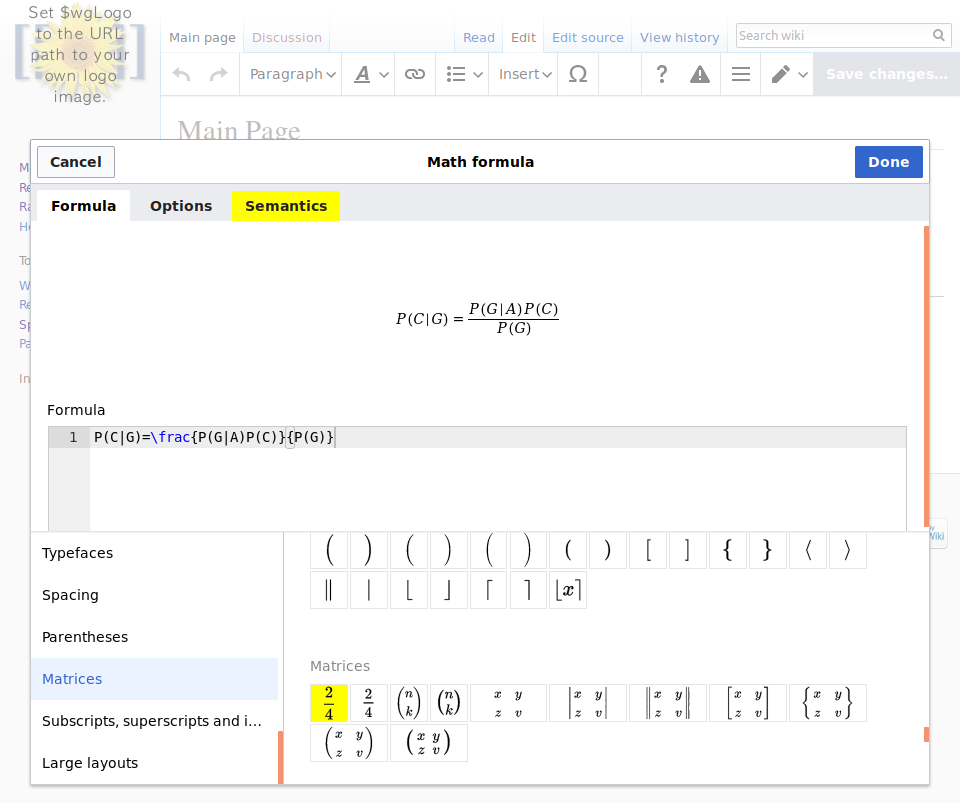
\includegraphics[width=\textwidth]{images/overview.png}
\caption{Math editing component of the VisualEditor.
 As of April 2018, users either need to know the LaTeX-command for `fraction' or use the fraction template ($\frac{2}{4}$, highlighted in yellow) and replace 2 by the numerator and 4 by the denominator of the formula.
 We will improve this dialog by adding semantic input as an alternative in the top panel (semantics, highlighted in yellow).}\label{fig.overview}
\end{figure}
\markdownInput{main.md}
\paragraph*{Acknowledgments} We thank the developers Ludwig Goohsen, Stefan Kaufhold, Jonas Kress, Vincent Stange and many others for their open source contributions.
 Furthermore, we thank the Wikimedia Foundation and in particular Thalia Chan, Ed Sanders and James Forrester from the editing team for the development of the current VisualEditor for Math.
\printbibliography[keyword=primary]
\end{document}
